\documentclass[12pt,a4paper]{article}
% Estilo compartido para informes. Compilar con LuaLaTeX desde tp1/.
\usepackage[spanish,es-nodecimaldot]{babel}
\usepackage{fontspec}
\setmainfont{Montserrat-Medium.ttf}[
  Path=../assets/fonts/,
  BoldFont=Montserrat-Bold.ttf,
  ItalicFont=Montserrat-MediumItalic.ttf]
\usepackage[a4paper,margin=2.5cm,headheight=16pt]{geometry}
\usepackage{xcolor,graphicx,booktabs,tabularx}
\usepackage{float}
\usepackage{titlesec,fancyhdr,enumitem,caption}
\usepackage{ragged2e}
\usepackage{hyperref}
\definecolor{verde}{HTML}{1D4036}
\definecolor{bronce}{HTML}{D38129}
\definecolor{rosa}{HTML}{D88E77}
\definecolor{calido}{HTML}{EFE4D8}
\definecolor{grafito}{HTML}{1D1D1D}
\hypersetup{colorlinks=true,linkcolor=verde,urlcolor=verde,
  pdftitle={TP1 - Instalación de máquinas virtuales},pdfsubject={Cyberseguridad}}
\AtBeginDocument{\color{grafito}\RaggedRight\fontsize{12}{14.4}\selectfont}
\setlength{\parindent}{0pt}
\setlength{\parskip}{7pt}
\setlist[itemize]{leftmargin=*,itemsep=7pt,topsep=4pt}
\setlist[enumerate]{leftmargin=*,itemsep=6pt}
\titleformat{\section}{\color{verde}\bfseries\fontsize{18}{21.6}\selectfont}{\thesection}{0.65em}{}
\titleformat{\subsection}{\color{verde}\bfseries\large}{\thesubsection}{0.65em}{}
\titleformat{\subsubsection}{\color{verde}\bfseries}{\thesubsubsection}{0.65em}{}
\titlespacing*{\section}{0pt}{16pt}{8pt}
\titlespacing*{\subsection}{0pt}{12pt}{5pt}
\titlespacing*{\subsubsection}{0pt}{10pt}{4pt}
\setcounter{tocdepth}{2}
\pagestyle{fancy}
\fancyhf{}
\fancyhead[L]{\small\color{verde}FCEFyN | UNC}
\fancyhead[R]{\small\color{verde}\materia\ · TP \numeroTP}
\fancyfoot[L]{\scriptsize Informe de laboratorio}
\fancyfoot[R]{\small\thepage}
\renewcommand{\headrulewidth}{0.4pt}
\captionsetup{font=small,labelfont=bf,justification=raggedright,singlelinecheck=false,hypcap=false}
\newcommand{\pendiente}[1]{\par{\small\color{verde}\textbf{Por completar.} #1\par}}
% Si falta una captura se muestra un espacio reservado; no impide compilar.
\newcommand{\captura}[2]{%
  \par\smallskip\begingroup\centering
  \IfFileExists{figuras/#1}{%
    \includegraphics[width=\linewidth,height=5cm,keepaspectratio]{figuras/#1}%
  }{%
    \setlength{\fboxsep}{10pt}%
    \fcolorbox{bronce}{calido}{\parbox[c][1.25cm][c]{\dimexpr\linewidth-2\fboxsep-2\fboxrule\relax}{%
      \centering\small Captura pendiente\par\texttt{\detokenize{#1}}}}%
  }%
  \captionof{figure}{#2}\par\endgroup\smallskip
}

\usepackage{xurl}

\newcommand{\materia}{Cyberseguridad}
\newcommand{\numeroTP}{2}
\newcommand{\tituloTP}{Registros de eventos}
\newcommand{\estudiante}{Brigido Tomas Andres}
\newcommand{\legajo}{38481096}
\newcommand{\carrera}{ICOMP}
\newcommand{\docente}{Javier A. Jorge}


% Metadatos específicos del TP2 y capturas en img/.
\hypersetup{pdftitle={TP2 - Registros de eventos}}
\renewcommand{\captura}[2]{%
  \begin{figure}[H]
    \centering
    \IfFileExists{img/#1}{%
      \includegraphics[width=0.85\linewidth,height=5cm,keepaspectratio]{img/#1}%
    }{%
      \setlength{\fboxsep}{10pt}%
      \fcolorbox{bronce}{calido}{\parbox[c][1.1cm][c]{0.85\linewidth}{%
        \centering\small Captura pendiente\par\texttt{\detokenize{#1}}}}%
    }%
    \caption{#2}
  \end{figure}
}

\begin{document}
\hypersetup{pageanchor=false}
\begin{titlepage}
  
\includegraphics[width=8cm]{../assets/logo-fcefyn-2026.png}
  \vspace{1cm}

  {\color{verde}\small UNIVERSIDAD NACIONAL DE CÓRDOBA\par}
  \vspace{2.1cm}
  {\color{bronce}\bfseries\large TRABAJO PRÁCTICO \numeroTP\par}
  \vspace{0.45cm}
  {\color{verde}\bfseries\fontsize{32}{38.4}\selectfont Registros de\\eventos\par}
  \vspace{0.65cm}
  {\large \materia\par}
  \vspace{0.8cm}
  {\color{bronce}\rule{2.7cm}{2pt}\par}
  \vfill
  \renewcommand{\arraystretch}{1.45}
  \begin{tabular}{@{}p{3.2cm}p{10cm}@{}}
    Estudiante & \estudiante \\
    Legajo & \legajo \\
    Carrera & \carrera \\
    Docente & \docente \\
  \end{tabular}
  \vfill
  {\small Córdoba, Argentina\par}
\end{titlepage}
\hypersetup{pageanchor=true}

\tableofcontents
\vspace{1cm}
\newpage

\section{Introducción y objetivos}
Este trabajo aborda la lectura, localización y monitoreo de registros de
 eventos en Linux mediante la máquina virtual CyberOps Workstation.
La práctica utiliza registros de servidores web y del sistema operativo
para ejercitar la interpretación de eventos y la búsqueda de evidencias.

\begin{itemize}
    \item Interpretar los campos de registros web y del sistema.
    \item Localizar la configuración y los archivos de registro de nginx.
    \item Observar eventos en tiempo real con \texttt{tail} y \texttt{journalctl}.
\end{itemize}

\section{Parte 1: descripción general de los registros}
\subsection{Registro de un servidor web}
\textbf{Interpretación de la entrada de Apache (p. 1 de la consigna).}

Lo que se puede interpretar del registro mostrado es que un cliente (el cual podemos ver si direccion ip)
hizo una peticion al servidor web de un arhcivo que no existe llamado \texttt{favicon.ico} y esto genero el error.

\textbf{Lectura del archivo de muestra.}
\begin{verbatim}
cat /var/log/logstash-tutorial.log
\end{verbatim}

Si se puede considerar una transaccion web ya que podemos ver el comando \texttt{GET} que es el que se utiliza para solicitar un recurso al servidor web.

El ejemplo muestra tres transacciones web, cada una con su fecha y hora, la direccion ip del cliente, el comando utilizado, el recurso solicitado y el codigo de respuesta del servidor.

La diferencia con el registro anterior es que el comando cat muestra todas las entradas del archivo de registro, mientras que el ejemplo de la consigna anterior solo muestra una entrada.
\subsection{Registro del sistema operativo}
\begin{verbatim}
sudo more /var/log/messages
\end{verbatim}

\textbf{Análisis de la lentitud de red reportada.}

Las entradas muestran pérdidas y recuperaciones del enlace de la interfaz enp0s3, indicadas mediante los mensajes “link down” y “link up”. Esto evidencia inestabilidad en la conexión. Sin embargo, corresponden al 20 de marzo, por lo que no permiten confirmar el problema reportado para el 19 de mayo a las 04:20.
\newpage
\section{Parte 2: ubicación de los registros de nginx}
\subsection{Documentación y procesos}

\begin{figure}[H]
    \centering
    \begin{minipage}[t]{0.48\textwidth}
        \centering
        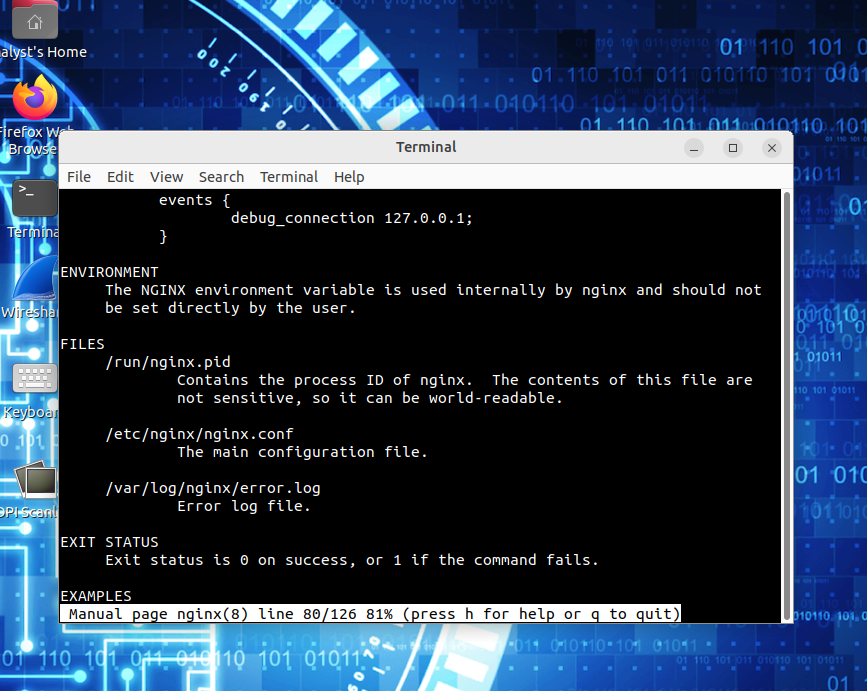
\includegraphics[width=\linewidth]{img/ngingxpath.png}
        \caption{Ruta de instalación de nginx.}
        \label{fig:imagen1}
    \end{minipage}
    \hfill
    \begin{minipage}[t]{0.48\textwidth}
        \centering
        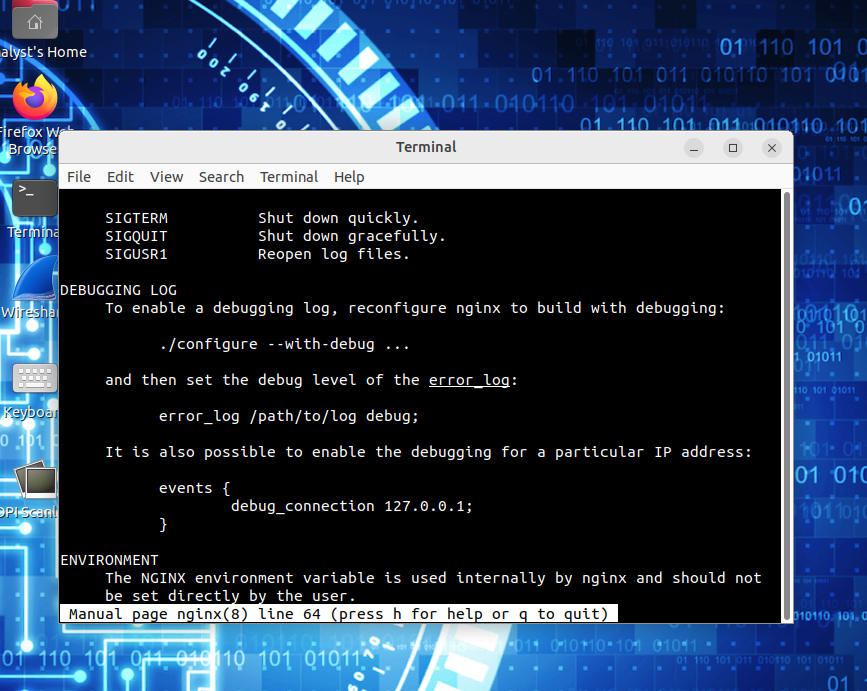
\includegraphics[width=\linewidth]{img/mannginx.png}
        \caption{Files de nginx.}
        \label{fig:imagen2}
    \end{minipage}
\end{figure}
 
\subsection{Búsqueda de la configuración y los archivos}
\begin{figure}[H]
    \centering
    \begin{minipage}[t]{0.48\textwidth}
        \centering
        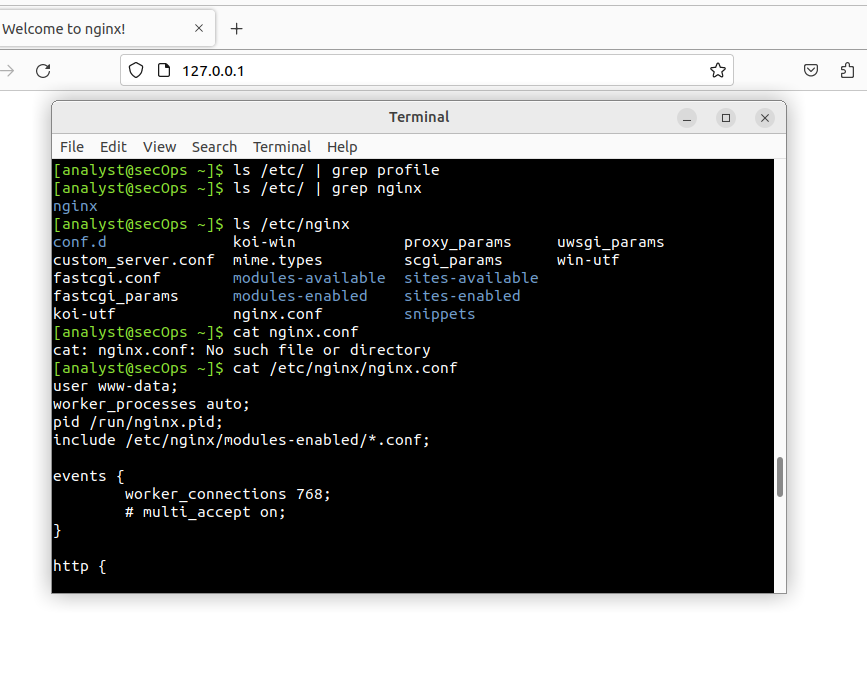
\includegraphics[width=\linewidth]{img/encontrandoNGINX.png}
        \caption{Files de configuración de nginx.}
        \label{fig:imagen1}
    \end{minipage}
    \hfill
    \begin{minipage}[t]{0.48\textwidth}
        \centering
        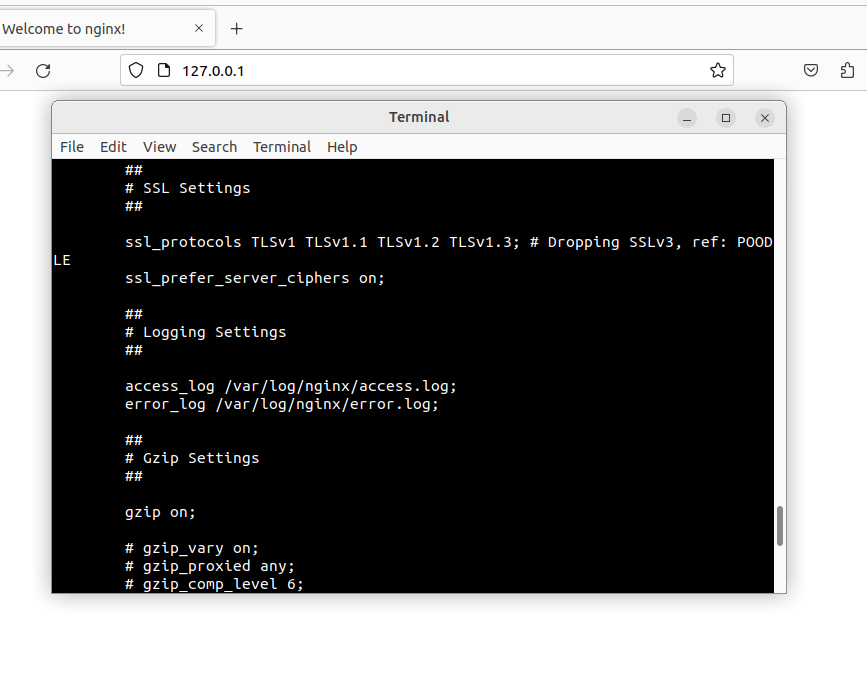
\includegraphics[width=\linewidth]{img/CARPETASNGINX.png}
        \caption{Carpetas de registro de nginx.}
        \label{fig:imagen2}
    \end{minipage}
    \hfill
    \begin{minipage}[t]{0.48\textwidth}
        \centering
        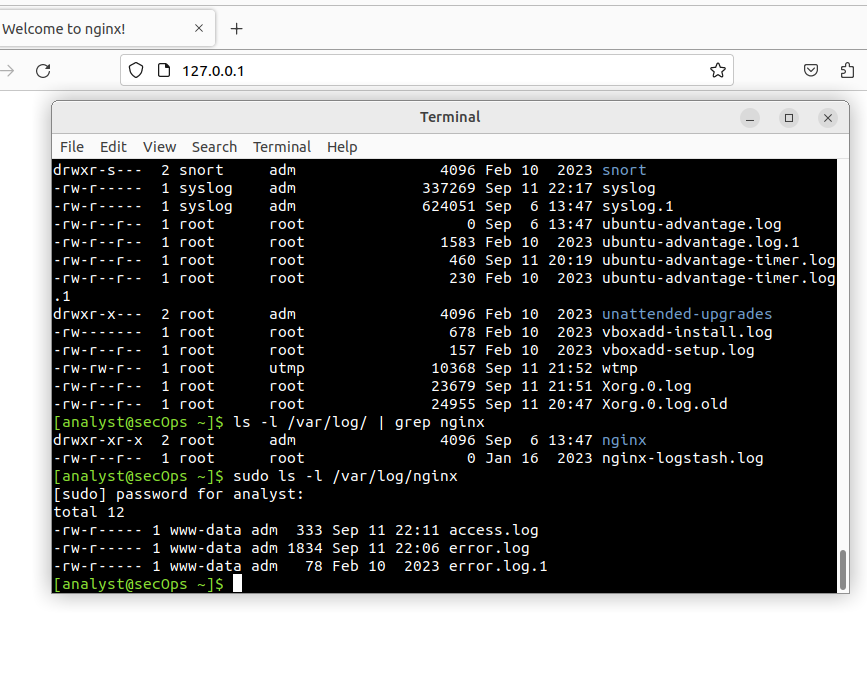
\includegraphics[width=\linewidth]{img/errorng.png}
        \caption{Logs de error de nginx.}
        \label{fig:imagen2}
    \end{minipage}
\end{figure}

\newpage
\section{Parte 3: monitoreo en tiempo real}
\subsection{Uso de tail}
\begin{figure}[H]
    \centering
    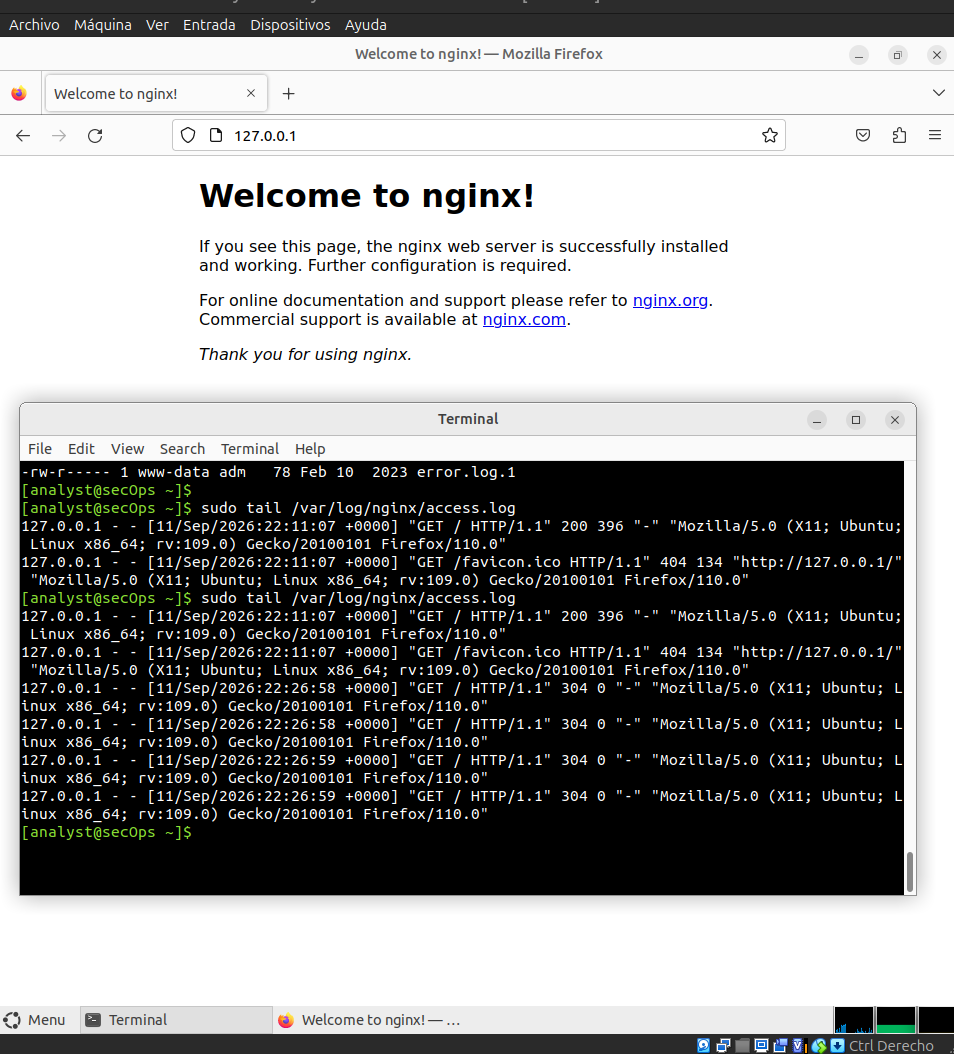
\includegraphics[width=0.85\textwidth]{img/tail.png}
    \caption{Monitoreo de access.log con tail.}
    \label{fig:imagen}
\end{figure}

Se utilizo las banderas -n y -f para mostrar las ultimas n lineas y para mostrar constanteme las lineas nuevas que se agregan al archivo de registro. Se observo que al acceder a la pagina web desde el navegador, se generaron nuevas entradas en el archivo access.log, lo que indica que el servidor web esta recibiendo y procesando las solicitudes de los clientes.

\subsection{Consulta del diario con journalctl}
\begin{verbatim}
journalctl
\end{verbatim}
\textbf{¿Cómo consultar todas las entradas disponibles del sistema?}

Para consultar todas las entradas disponibles del sistema, se puede ejecutar el comando \texttt{sudo journalctl}.
\begin{figure}[H]
    \centering
    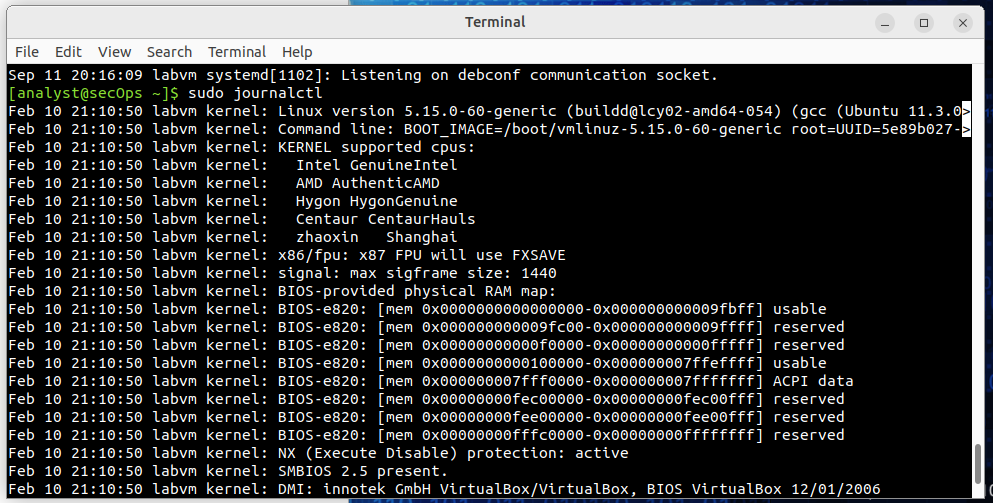
\includegraphics[width=0.85\textwidth]{img/ctlconsudo.png}
    \caption{Consulta del diario con journalctl.}
    \label{fig:imagen}
\end{figure}
\subsection{Filtros por arranque, tiempo y servicio}
\begin{verbatim}
sudo journalctl -b
sudo journalctl -b -1
sudo journalctl -b -2
sudo journalctl --list-boots
sudo journalctl --since "2 hours ago"
sudo journalctl --since "1 day ago"
sudo journalctl -u nginx.service
\end{verbatim}

\begin{figure}[H]
    \centering
    \begin{minipage}[t]{0.48\textwidth}
        \centering
        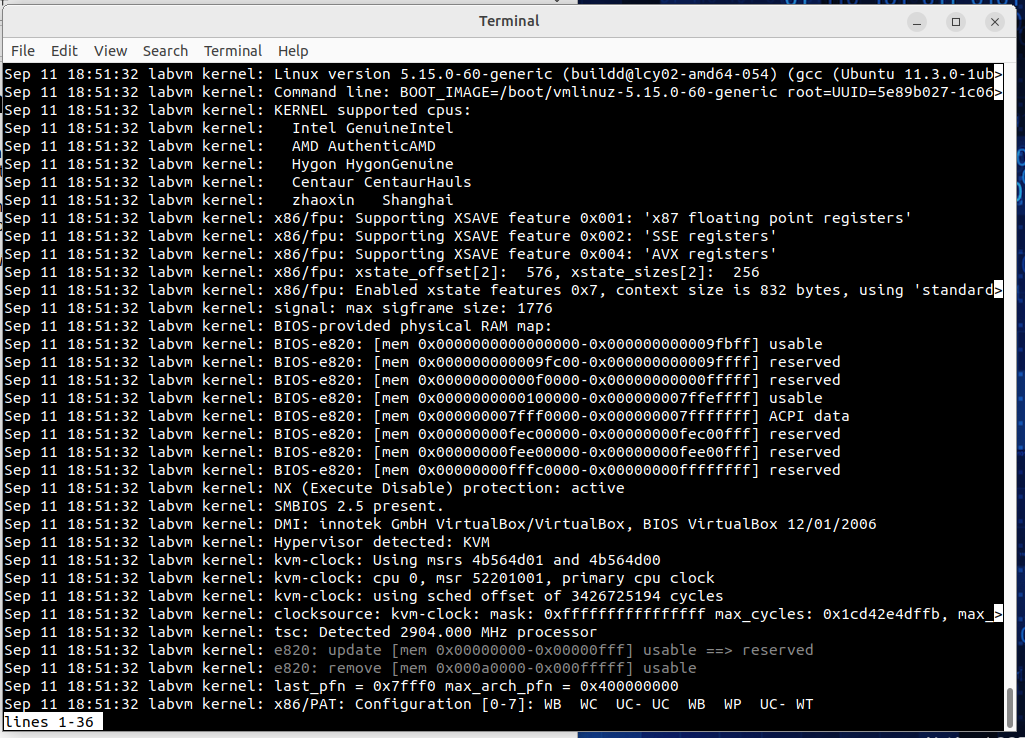
\includegraphics[width=\linewidth]{img/flagB.png}
        \caption{Consulta del diario con journalctl y la bandera -b.}
        \label{fig:imagen1}
    \end{minipage}
    \hfill
    \begin{minipage}[t]{0.48\textwidth}
        \centering
        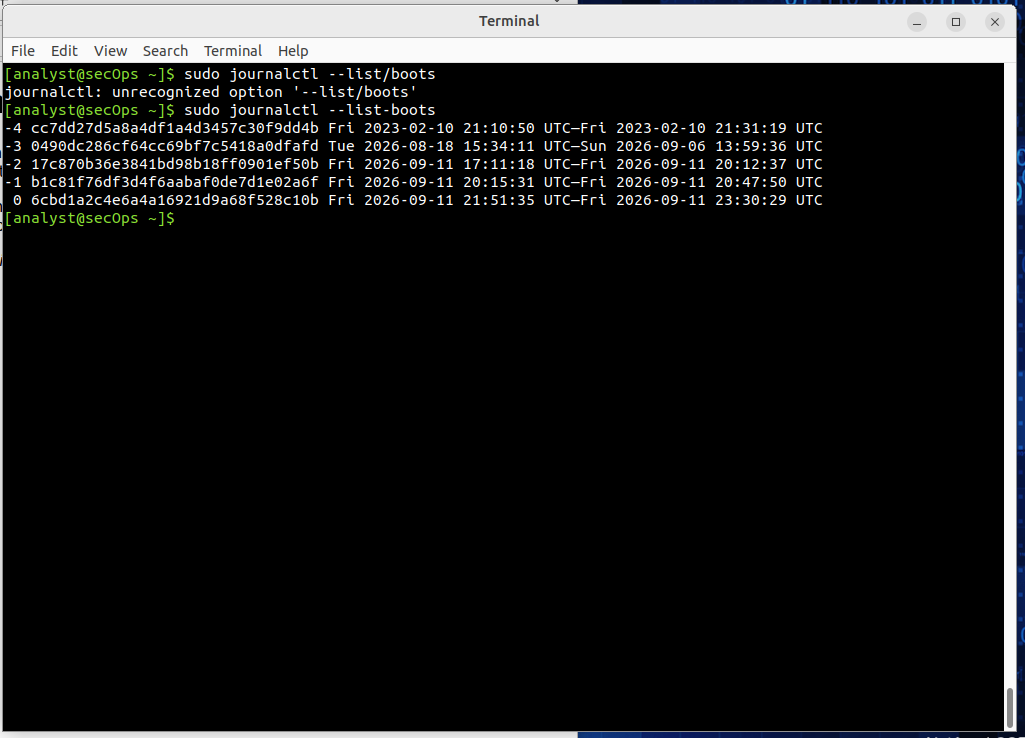
\includegraphics[width=\linewidth]{img/bootsflags.png}
        \caption{Filtros por arranque.}
        \label{fig:imagen2}
    \end{minipage}
    \hfill
    \begin{minipage}[t]{0.48\textwidth}
        \centering
        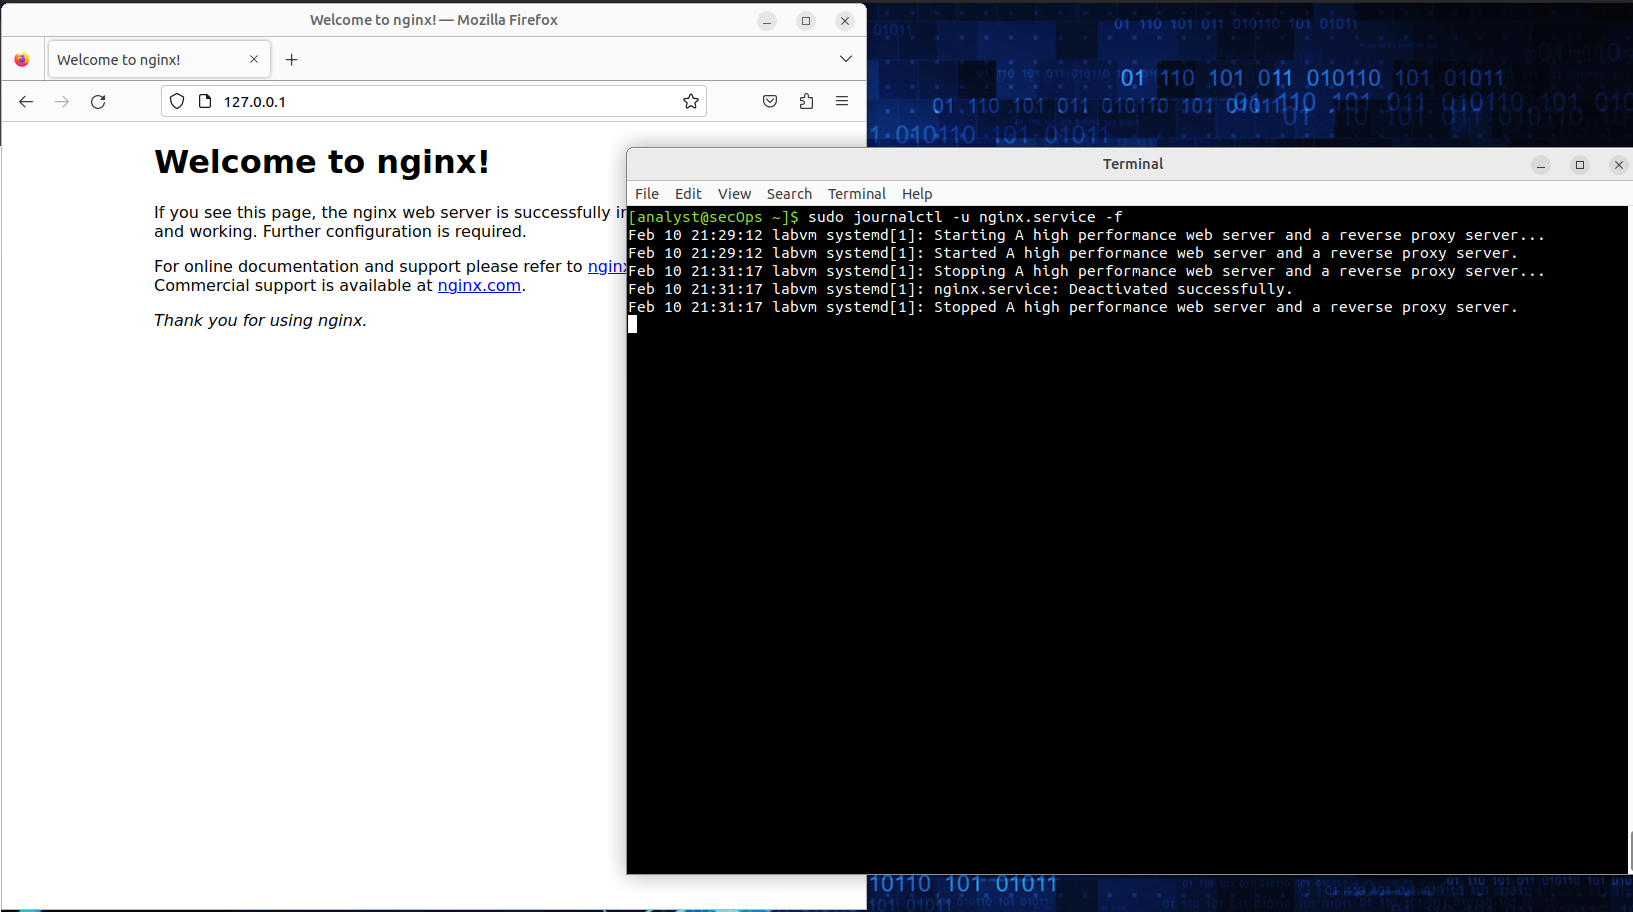
\includegraphics[width=\linewidth]{img/nginxconf.png}
        \caption{Logs con bandera de seguimiento.}
        \label{fig:imagen2}
    \end{minipage}
\end{figure}


\section{Reflexión}
Como reflexion puedo decir que a la hora de detectar amenzas y errores,
los archivos de configuracion y los archivos de registro son muy importantes ya que nos permiten ver que esta pasando en el sistema.
Estos archivos junto con las herramientas de monitoreo de red nos permiten detectar problemas e incluso intrusos
en nuestro sistema. Por lo tanto, es importante conocer la ubicacion de estos archivos y como interpretarlos para poder mantener la seguridad de nuestro sistema.

Otra reflexion importante es la de tener en cuenta los relojes de los sistemas. Los relojes siempre deben estar sincronizados para garantizar que todos los sistemas tengan la hora
correcta. Si los relojes no están definidos correctamente, es muy difícil realizar un retroseguimiento de los
eventos.

\newpage
\section{Referencias}
\begin{enumerate}
    \item Cisco Networking Academy. \textit{Práctica de laboratorio:
    Registros de eventos}, 2017--2020. Consigna suministrada en
    \textit{2B Trabajo con archivos de registro de evento.pdf}, 17 páginas.
    \item FCEFyN, Universidad Nacional de Córdoba. \textit{Manual de
    identidad visual}, 2026. Base del estilo compartido del informe.
\end{enumerate}
\end{document}
